\documentclass[10pt,letterpaper]{article}

\usepackage[top=0.8in,bottom=0.8in,left=0.8in,right=0.8in]{geometry}
\usepackage[utf8]{inputenc}
\usepackage[T1]{fontenc}
\usepackage{lmodern}
\usepackage{microtype}
\usepackage{amsmath,amsfonts,amssymb}
\usepackage{booktabs}
\usepackage{tabularx}
\usepackage{longtable}
\usepackage{array}
\usepackage{xcolor}
\usepackage{listings}
\usepackage{fancyhdr}
\usepackage{titlesec}
\usepackage{enumitem}
\usepackage{parskip}
\usepackage{tikz}
\usetikzlibrary{shapes.geometric,arrows.meta,positioning,fit,backgrounds,calc}

% Define color palette
\definecolor{primary}{HTML}{1A365D}
\definecolor{secondary}{HTML}{2B6CB0}
\definecolor{accent}{HTML}{319795}
\definecolor{darkgray}{HTML}{2D3748}
\definecolor{lightgray}{HTML}{F7FAFC}
\definecolor{bordergray}{HTML}{E2E8F0}
\definecolor{codebg}{HTML}{F8FAFC}
\definecolor{codeborder}{HTML}{E2E8F0}
\definecolor{kwcolor}{HTML}{805AD5}
\definecolor{strcolor}{HTML}{2C7A7B}
\definecolor{comcolor}{HTML}{718096}

\usepackage[colorlinks=true,
            linkcolor=secondary,
            citecolor=secondary,
            urlcolor=secondary]{hyperref}

% Header and Footer
\pagestyle{fancy}
\fancyhf{}
\fancyhead[L]{\textsf{\footnotesize \textbf{DATA 607 Group Project} $\vert$ Data Ingestion Pipeline Architecture}}
\fancyhead[R]{\textsf{\footnotesize October 2026}}
\fancyfoot[C]{\textsf{\thepage}}
\renewcommand{\headrulewidth}{0.4pt}
\renewcommand{\footrulewidth}{0.4pt}

% Section formatting
\titleformat{\section}
  {\Large\bfseries\sffamily\color{primary}}
  {\thesection}{1em}{}
  [{\color{primary}\titlerule[1pt]}]

\titleformat{\subsection}
  {\large\bfseries\sffamily\color{secondary}}
  {\thesubsection}{1em}{}

\titleformat{\subsubsection}
  {\normalsize\bfseries\sffamily\color{darkgray}}
  {\thesubsubsection}{1em}{}

% Listings configuration
\lstset{
  backgroundcolor=\color{codebg},
  basicstyle=\ttfamily\footnotesize\color{darkgray},
  breaklines=true,
  breakatwhitespace=true,
  frame=single,
  rulecolor=\color{codeborder},
  keywordstyle=\bfseries\color{kwcolor},
  stringstyle=\color{strcolor},
  commentstyle=\itshape\color{comcolor},
  numbers=none,
  tabsize=2,
  showstringspaces=false,
  captionpos=b,
  keepspaces=true
}

\begin{document}

\begin{titlepage}
    \centering
    \vspace*{1.5cm}
    
    {\Huge \bfseries \sffamily \color{primary} Multi-Source Job Market\\[0.3em] Data Ingestion Engine}\\[1.5em]
    {\Large \sffamily \color{secondary} Comprehensive Code Audit \& System Architecture Documentation}\\[2.5em]
    
    \rule{0.6\textwidth}{1.2pt}\\[2.5em]
    
    \begin{minipage}{0.8\textwidth}
        \sffamily \normalsize
        \textbf{Course:} DATA 607 -- Data Acquisition and Management\\
        \textbf{Repository:} \texttt{data\_ingestion}\\
        \textbf{Domain:} Job Board Telemetry, Normalization \& Relational ETL\\
        \textbf{Target Storage:} Local SQLite (\texttt{jobs.db}) / Cloud PostgreSQL (\texttt{Neon})\\
        \textbf{Execution Engine:} Windows Task Scheduler / Python 3.11 Orchestrator\\
        \textbf{Date:} October 2026 $\vert$ Version 1.0.0
    \end{minipage}
    
    \vfill
    
    {\small \textsf{Production-Grade Software Architecture \& Engineering Audit}}
    \vspace*{1cm}
\end{titlepage}

\tableofcontents
\newpage

% ============================================================================
% SECTION 1
% ============================================================================
\section{Repository \& Directory Walkthrough}

\subsection{Directory Tree Overview}

The repository follows a clean, modular structure separating configuration, extraction clients (fetchers), record transformation (parsers), relational database persistence (loaders), and automated scheduled task runners.

\begin{lstlisting}[language=bash, caption={Hierarchical Repository Layout}]
data_ingestion/
|-- config/
|   `-- sources.yaml                # Declarative endpoint, rate limit & schema configs
|-- data/
|   |-- db/
|   |   `-- jobs.db                 # Local SQLite database target
|   `-- raw/                        # Date-partitioned raw payload landing zone
|       |-- adzuna/<date>/data.json
|       |-- arbeitnow/<date>/data.json
|       |-- himalayas/<date>/data.json
|       |-- hn_hiring/<date>/data.json
|       |-- jobicy/<date>/data.json
|       |-- remoteok/<date>/data.json
|       |-- usajobs/<date>/data.json
|       `-- wwr/<date>/data.json
|-- logs/
|   |-- pipeline_YYYY-MM-DD.log     # Daily run logs and load metrics
|   `-- source_health_YYYY-MM-DD.json # Pre-flight diagnostic telemetry
|-- scripts/
|   |-- check_sources.py            # Diagnostic liveness, schema & robots.txt auditor
|   `-- run_daily.ps1               # Scheduled Task PowerShell wrapper
|-- src/
|   |-- pipeline.py                 # Core CLI orchestrator
|   |-- db/
|   |   |-- __init__.py             # DB module init
|   |   |-- load.py                 # SQLite idempotent persistence backend
|   |   |-- load_postgres.py        # PostgreSQL (Neon) persistence backend
|   |   |-- schema.sql              # Normalized SQLite DDL schema
|   |   `-- schema_postgres.sql     # Normalized PostgreSQL DDL schema
|   |-- fetchers/                   # Source extraction clients (HTTP/RSS/Algolia)
|   |   |-- __init__.py
|   |   |-- base.py                 # Throttling, retry/backoff & User-Agent plumbing
|   |   |-- adzuna.py, arbeitnow.py, himalayas.py, hn_hiring.py
|   |   `-- jobicy.py, remoteok.py, usajobs.py, wwr.py
|   `-- parsers/                    # Field normalization & quality validation
|       |-- __init__.py             # Canonical ROW_FIELDS and validator
|       |-- adzuna.py, arbeitnow.py, himalayas.py, hn_hiring.py
|       `-- jobicy.py, remoteok.py, usajobs.py, wwr.py
|-- tests/
|   |-- conftest.py, test_db_load.py, test_parsers.py
|   |-- test_rate_limit.py, test_retry.py
|   `-- fixtures/                   # Offline test payload snapshots
`-- requirements.txt                # Third-party Python dependencies
\end{lstlisting}

\subsection{Folder-by-Folder Responsibilities}

\begin{table}[htbp]
\centering
\small
\begin{tabularx}{\textwidth}{p{3.2cm}X}
\toprule
\textbf{Folder Path} & \textbf{Role within the Ingestion Lifecycle} \\
\midrule
\texttt{config/} & \textbf{Configuration Layer:} Houses declarative YAML files specifying ingestion endpoints, rate-limiting constraints, access credentials, and expected schema contracts. \\
\addlinespace
\texttt{scripts/} & \textbf{Operations \& Automation:} Contains operational automation utilities, including pre-flight source health audits and scheduled execution wrappers for Windows Task Scheduler. \\
\addlinespace
\texttt{src/} & \textbf{Core Pipeline Package:} Contains the central CLI pipeline orchestrator coordinating extraction, disk staging, normalization, validation, and multi-backend loading. \\
\addlinespace
\texttt{src/fetchers/} & \textbf{Extraction Layer:} Encapsulates protocol-specific network communication (REST, RSS XML, Algolia API) with respectful monotonic throttling and Tenacity exponential backoff. \\
\addlinespace
\texttt{src/parsers/} & \textbf{Transformation \& Quality Layer:} Maps heterogeneous raw schemas to a uniform 13-column relational contract and validates data types and URL integrity. \\
\addlinespace
\texttt{src/db/} & \textbf{Persistence Layer:} Implements 3NF normalized DDL schemas and idempotent upsert drivers for both SQLite and PostgreSQL (Neon). \\
\addlinespace
\texttt{data/raw/} & \textbf{Data Lake / Raw Staging:} Immutable date-partitioned landing zone where verbatim JSON/XML API responses are snapshotted prior to transformation. \\
\addlinespace
\texttt{data/db/} & \textbf{Storage Target:} Dedicated directory storing the active SQLite database file (\texttt{jobs.db}). \\
\addlinespace
\texttt{logs/} & \textbf{Telemetry \& Observability:} Centralized log directory recording execution timestamps, pipeline summary tables, and JSON health reports. \\
\addlinespace
\texttt{tests/} & \textbf{Quality Assurance:} Unit and integration test suites validating parsers, rate limiting, retries, and database idempotency against recorded fixtures. \\
\bottomrule
\end{tabularx}
\caption{System Directory Responsibilities}
\end{table}

\subsection{File-by-File Breakdown}

\subsubsection{Configuration and Scripts}
\begin{itemize}[leftmargin=1.5em]
    \item \textbf{\texttt{config/sources.yaml}:} Source configuration manifest. Declares endpoint URLs, rate limits, access types, credential environment variables, and pre-parse required fields for 8 sources.
    \item \textbf{\texttt{scripts/check\_sources.py}:} Standalone pre-flight auditor. Assesses API liveness, measures response latency, validates schema contracts against live payloads, checks \texttt{robots.txt} compliance, and writes telemetry to \texttt{logs/source\_health\_<date>.json}.
    \item \textbf{\texttt{scripts/run\_daily.ps1}:} Production PowerShell task runner. Triggered by Windows Task Scheduler, invokes the pipeline orchestrator, logs execution output, and preserves exit codes.
\end{itemize}

\subsubsection{Orchestration \& Core Engine}
\begin{itemize}[leftmargin=1.5em]
    \item \textbf{\texttt{src/pipeline.py}:} Master orchestrator. Iterates over active sources, coordinates fetchers, writes raw payloads to disk, executes parsers and validation, and commits batches to the selected database backend. Entry functions: \texttt{main()}, \texttt{run\_source()}.
\end{itemize}

\subsubsection{Fetchers (\texttt{src/fetchers/})}
\begin{itemize}[leftmargin=1.5em]
    \item \textbf{\texttt{base.py}:} Shared networking infrastructure. Provides monotonic interval throttling (\texttt{throttle()}), project-identified User-Agent generation (\texttt{build\_headers()}), and Tenacity exponential retries (\texttt{get()}) targeting HTTP 429 and 5xx errors.
    \item \textbf{\texttt{remoteok.py}:} RemoteOK REST client. Fetches complete unpaginated listings, filtering out the initial metadata notice.
    \item \textbf{\texttt{arbeitnow.py}:} Arbeitnow REST client. Retrieves active postings under the \texttt{"data"} response key.
    \item \textbf{\texttt{jobicy.py}:} Jobicy API v2 client. Implements sample queries (\texttt{count=5}) and batch extractions (\texttt{count=50}).
    \item \textbf{\texttt{himalayas.py}:} Himalayas REST client. Executes batch queries with parameterized limits (\texttt{limit=100}).
    \item \textbf{\texttt{wwr.py}:} We Work Remotely RSS client. Downloads XML feeds and parses feed entries using \texttt{feedparser}.
    \item \textbf{\texttt{hn\_hiring.py}:} Hacker News Algolia client. Dynamically resolves the latest "Ask HN: Who is hiring" monthly thread ID, then fetches child comments (up to 1,000 hits).
    \item \textbf{\texttt{adzuna.py}:} Authenticated Adzuna API client. Verifies \texttt{ADZUNA\_APP\_ID} and \texttt{ADZUNA\_APP\_KEY} to fetch US data science postings.
    \item \textbf{\texttt{usajobs.py}:} Authenticated USAJobs REST client. Utilizes \texttt{USAJOBS\_API\_KEY} and \texttt{USAJOBS\_EMAIL}, flattening nested \texttt{MatchedObjectDescriptor} structures.
\end{itemize}

\subsubsection{Parsers (\texttt{src/parsers/})}
\begin{itemize}[leftmargin=1.5em]
    \item \textbf{\texttt{\_\_init\_\_.py}:} Schema contract definition. Declares \texttt{ROW\_FIELDS}, implements \texttt{empty\_row()}, and enforces pre-load validation (\texttt{validate\_row()}) checking mandatory keys and URL structure.
    \item \textbf{Source Parsers (\texttt{remoteok.py}, \texttt{arbeitnow.py}, etc.):} Map source-specific attributes to the uniform 13-field record. Converts Unix epoch times to ISO UTC strings (\texttt{arbeitnow}), splits composite company-title strings (\texttt{wwr}), stores free-text comments verbatim without speculative inference (\texttt{hn\_hiring}), and safely parses numerical salary bounds (\texttt{usajobs}).
\end{itemize}

\subsubsection{Database Loaders (\texttt{src/db/})}
\begin{itemize}[leftmargin=1.5em]
    \item \textbf{\texttt{schema.sql} \& \texttt{schema\_postgres.sql}:} Normalized 3NF DDL definitions for \texttt{sources}, \texttt{companies}, \texttt{jobs}, \texttt{tags}, and \texttt{job\_tags}.
    \item \textbf{\texttt{load.py}:} SQLite persistence driver. Connects, applies DDL migrations, and performs idempotent upserts using \texttt{ON CONFLICT(source\_id, external\_id) DO UPDATE}.
    \item \textbf{\texttt{load\_postgres.py}:} PostgreSQL/Neon persistence driver. Implements identical idempotent loading semantics using \texttt{psycopg} and \texttt{\%s} parameterized placeholders.
\end{itemize}

\newpage
% ============================================================================
% SECTION 2
% ============================================================================
\section{End-to-End Pipeline Architecture}

\subsection{Architecture Diagram}

\begin{figure}[htbp]
\centering
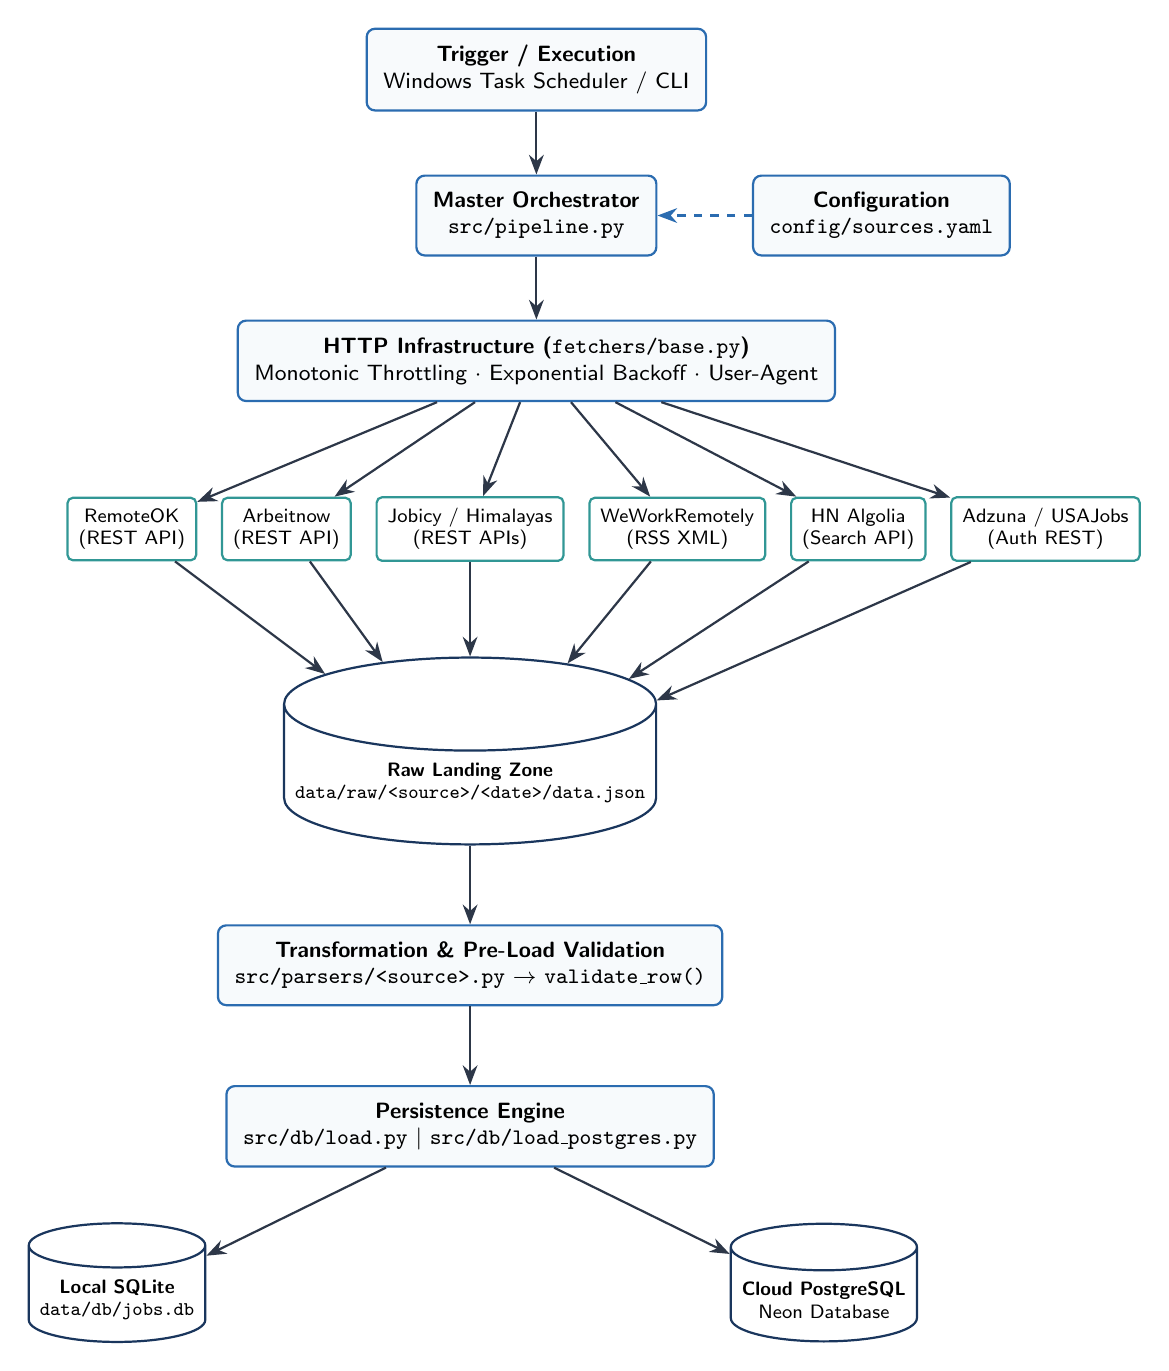
\begin{tikzpicture}[
    node distance=1.0cm and 1.2cm,
    box/.style={rectangle, draw=secondary, fill=lightgray, thick, rounded corners=3pt, align=center, font=\sffamily\footnotesize, inner sep=6pt},
    sourcebox/.style={rectangle, draw=accent, fill=white, thick, rounded corners=2pt, align=center, font=\sffamily\scriptsize, inner sep=4pt},
    dbbox/.style={cylinder, draw=primary, fill=white, thick, shape border rotate=90, aspect=0.25, align=center, font=\sffamily\scriptsize, inner sep=4pt},
    arrow/.style={-{Stealth[length=2.5mm]}, thick, color=darkgray},
    dasharrow/.style={-{Stealth[length=2.5mm]}, dashed, thick, color=secondary}
]

% Trigger Layer
\node[box, fill=codebg] (scheduler) {\textbf{Trigger / Execution}\\Windows Task Scheduler / CLI};
\node[box, below=0.8cm of scheduler] (orchestrator) {\textbf{Master Orchestrator}\\ \texttt{src/pipeline.py}};
\node[box, right=1.2cm of orchestrator] (config) {\textbf{Configuration}\\ \texttt{config/sources.yaml}};

% Networking
\node[box, below=0.8cm of orchestrator] (fetchbase) {\textbf{HTTP Infrastructure (\texttt{fetchers/base.py})}\\Monotonic Throttling $\cdot$ Exponential Backoff $\cdot$ User-Agent};

% Sources
\node[sourcebox, below left=1.2cm and 0.5cm of fetchbase] (src1) {RemoteOK\\(REST API)};
\node[sourcebox, right=0.3cm of src1] (src2) {Arbeitnow\\(REST API)};
\node[sourcebox, right=0.3cm of src2] (src3) {Jobicy / Himalayas\\(REST APIs)};
\node[sourcebox, right=0.3cm of src3] (src4) {WeWorkRemotely\\(RSS XML)};
\node[sourcebox, right=0.3cm of src4] (src5) {HN Algolia\\(Search API)};
\node[sourcebox, right=0.3cm of src5] (src6) {Adzuna / USAJobs\\(Auth REST)};

% Raw Staging
\node[dbbox, below=1.2cm of src3] (datalake) {\textbf{Raw Landing Zone}\\ \texttt{data/raw/<source>/<date>/data.json}};

% Normalization & Validation
\node[box, below=1.0cm of datalake] (parsers) {\textbf{Transformation \& Pre-Load Validation}\\ \texttt{src/parsers/<source>.py} $\to$ \texttt{validate\_row()}};

% Storage
\node[box, below=1.0cm of parsers] (loaders) {\textbf{Persistence Engine}\\ \texttt{src/db/load.py} $\vert$ \texttt{src/db/load\_postgres.py}};
\node[dbbox, below left=0.8cm and 0.5cm of loaders] (sqlite) {\textbf{Local SQLite}\\ \texttt{data/db/jobs.db}};
\node[dbbox, below right=0.8cm and 0.5cm of loaders] (postgres) {\textbf{Cloud PostgreSQL}\\ Neon Database};

% Connections
\draw[arrow] (scheduler) -- (orchestrator);
\draw[dasharrow] (config) -- (orchestrator);
\draw[arrow] (orchestrator) -- (fetchbase);
\draw[arrow] (fetchbase) -- (src1);
\draw[arrow] (fetchbase) -- (src2);
\draw[arrow] (fetchbase) -- (src3);
\draw[arrow] (fetchbase) -- (src4);
\draw[arrow] (fetchbase) -- (src5);
\draw[arrow] (fetchbase) -- (src6);

\draw[arrow] (src1) -- (datalake);
\draw[arrow] (src2) -- (datalake);
\draw[arrow] (src3) -- (datalake);
\draw[arrow] (src4) -- (datalake);
\draw[arrow] (src5) -- (datalake);
\draw[arrow] (src6) -- (datalake);

\draw[arrow] (datalake) -- (parsers);
\draw[arrow] (parsers) -- (loaders);
\draw[arrow] (loaders) -- (sqlite);
\draw[arrow] (loaders) -- (postgres);

\end{tikzpicture}
\caption{End-to-End Pipeline Architectural Dataflow}
\end{figure}

\subsection{Data Lifecycle Stages}

\begin{enumerate}[leftmargin=2em]
    \item \textbf{Ingestion Trigger:}
    Daily execution is triggered via Windows Task Scheduler executing \texttt{scripts/run\_daily.ps1}. Manual and ad-hoc runs are initiated via \texttt{python src/pipeline.py} with optional CLI filters (\texttt{--sources}, \texttt{--backend}).
    
    \item \textbf{Source Extraction:}
    Network requests are mediated by \texttt{src/fetchers/base.py}. Each source is queried using a pull-based REST API call or RSS parse. Rate limits (\texttt{rate\_limit\_sec}) and transparent User-Agent headers are enforced for polite data scraping.
    
    \item \textbf{Staging / Raw Persistence:}
    Before transformation, the raw upstream response payload is saved verbatim to:
    \[
        \texttt{data/raw/}\langle\text{source}\rangle/\langle\text{run\_date}\rangle/\texttt{data.json}
    \]
    This landing zone guarantees full auditability and enables offline parser replays.
    
    \item \textbf{Validation \& Transformation:}
    Payloads are mapped by source-specific parsers to the canonical \texttt{ROW\_FIELDS} contract. Records undergo quality validation (\texttt{validate\_row()}): required fields (\texttt{source}, \texttt{external\_id}, \texttt{retrieved\_at}) must be populated, and any \texttt{url} present must be syntactically valid with an HTTP/HTTPS scheme and network domain. Malformed records are discarded from the batch and logged.
    
    \item \textbf{Loading \& Destination:}
    Validated rows are loaded via \texttt{load.py} (SQLite) or \texttt{load\_postgres.py} (PostgreSQL). Entities are upserted into 3NF normalized tables (\texttt{sources}, \texttt{companies}, \texttt{jobs}, \texttt{tags}, \texttt{job\_tags}). Existing job records matching \texttt{(source\_id, external\_id)} are updated in place, ensuring full idempotency.
\end{enumerate}

\newpage
% ============================================================================
% SECTION 3
% ============================================================================
\section{Code Section \& Logic Breakdown}

\subsection{Logical Section 1: Orchestration \& Configuration}
\begin{itemize}[leftmargin=1.5em]
    \item \textbf{Related Files:} \texttt{src/pipeline.py}, \texttt{config/sources.yaml}
    \item \textbf{Detailed Mechanism:} The entry point \texttt{main()} parses runtime arguments and reads \texttt{sources.yaml}. For every configured source, \texttt{run\_source()} performs credential checks, invokes extraction, writes the raw snapshot to disk, iterates extracted records through parsers and validators, and executes database upserts. Transactions are committed per source (\texttt{conn.commit()}), providing transactional isolation.
    \item \textbf{Key Methods:}
    \begin{itemize}
        \item \texttt{run\_source(name, scfg, contact\_email, session, run\_date, conn, loader) -> dict}: Executes end-to-end ingestion for one source. Returns status dictionary containing metrics (\texttt{fetched}, \texttt{loaded}, \texttt{invalid}).
        \item \texttt{main()}: Coordinates source iteration, manages backend database connections, and outputs summary execution telemetry.
    \end{itemize}
    \item \textbf{Error Handling \& Resilience:} Network failures are trapped within \texttt{run\_source()}, returning \texttt{status: "fetch\_error"} without terminating other sources. Missing API credentials safely bypass execution with \texttt{status: "skipped\_no\_key"}.
\end{itemize}

\subsection{Logical Section 2: HTTP Infrastructure \& Politeness}
\begin{itemize}[leftmargin=1.5em]
    \item \textbf{Related Files:} \texttt{src/fetchers/base.py}
    \item \textbf{Detailed Mechanism:}
    Maintains a monotonic timestamp registry \texttt{\_last\_call\_at} per \texttt{rate\_key}. \texttt{throttle()} pauses execution via \texttt{time.sleep()} if the elapsed time since the previous call is less than \texttt{min\_interval\_sec}. Wraps HTTP GET in a Tenacity retry handler configured with exponential backoff:
    \begin{lstlisting}[language=Python]
@retry(
    stop=stop_after_attempt(4),
    wait=wait_exponential(multiplier=1, min=1, max=10),
    retry=retry_if_exception(_is_retryable),
    reraise=True,
)
def get(session, url, *, rate_key, min_interval_sec, timeout=15, **kwargs):
    throttle(rate_key, min_interval_sec)
    resp = session.get(url, timeout=timeout, **kwargs)
    resp.raise_for_status()
    return resp
    \end{lstlisting}
    \item \textbf{Error Handling \& Resilience:} The \texttt{\_is\_retryable()} predicate retries only on HTTP 429 (rate-limited) and 5xx (transient gateway/server errors). Fatal client errors (e.g., 401, 403, 404) fail immediately.
\end{itemize}

\subsection{Logical Section 3: Source Extractors (Fetchers)}
\begin{itemize}[leftmargin=1.5em]
    \item \textbf{Related Files:} \texttt{src/fetchers/remoteok.py}, \texttt{arbeitnow.py}, \texttt{jobicy.py}, \texttt{himalayas.py}, \texttt{wwr.py}, \texttt{hn\_hiring.py}, \texttt{adzuna.py}, \texttt{usajobs.py}
    \item \textbf{Detailed Mechanism:} Each module implements \texttt{fetch\_all(session, cfg)} and \texttt{fetch\_sample(session, cfg)}.
    \begin{itemize}
        \item \emph{RemoteOK:} Drops the leading non-job legal/notice item from the raw JSON array.
        \item \emph{WeWorkRemotely:} Employs \texttt{feedparser} to parse RSS XML feeds into uniform entry dictionaries.
        \item \emph{HN Hiring:} Implements a two-step query against the Algolia Search API. Queries \texttt{tags=story\&query=Who is hiring} to locate the latest monthly parent thread ID, then fetches child comments up to Algolia's limit of 1,000 hits.
        \item \emph{Adzuna \& USAJobs:} Authenticate via query parameters and custom request headers, flattening deeply nested structures.
    \end{itemize}
\end{itemize}

\subsection{Logical Section 4: Data Normalization \& Quality Validation}
\begin{itemize}[leftmargin=1.5em]
    \item \textbf{Related Files:} \texttt{src/parsers/\_\_init\_\_.py}, and source-specific parsers
    \item \textbf{Canonical Contract:} Every parser instantiates rows conforming to:
    \begin{lstlisting}[language=Python]
ROW_FIELDS = (
    "source", "external_id", "title", "company", "location", "remote_type",
    "posted_date", "retrieved_at", "url", "salary_min", "salary_max",
    "description_raw", "tags_raw",
)
    \end{lstlisting}
    \item \textbf{Validation Logic:} \texttt{validate\_row(row)} ensures \texttt{source}, \texttt{external\_id}, and \texttt{retrieved\_at} are non-null and checks that any provided \texttt{url} satisfies RFC URI standards via \texttt{urllib.parse.urlparse}.
    \item \textbf{Zero-Inference Policy:} In accordance with data integrity guidelines, free-text sources (such as Hacker News comments) are captured verbatim in \texttt{description\_raw} without applying speculative regex heuristics to infer job title or company.
\end{itemize}

\subsection{Logical Section 5: Relational Persistence \& Multi-Backend Loading}
\begin{itemize}[leftmargin=1.5em]
    \item \textbf{Related Files:} \texttt{src/db/load.py}, \texttt{load\_postgres.py}, \texttt{schema.sql}, \texttt{schema\_postgres.sql}
    \item \textbf{Detailed Mechanism:} On connection, the schema DDL is executed with \texttt{CREATE TABLE IF NOT EXISTS}. Rows are loaded through an idempotent normalization sequence:
    \begin{enumerate}
        \item \texttt{get\_or\_create\_source()}: Upserts source name and base URL.
        \item \texttt{get\_or\_create\_company()}: Inserts company name (\texttt{ON CONFLICT DO NOTHING}).
        \item \texttt{upsert\_job()}: Inserts job record on composite natural key \texttt{UNIQUE(source\_id, external\_id)}. On conflict, all mutable fields (dates, salary, description) are updated in place, returning \texttt{job\_id}.
        \item \texttt{upsert\_tags()}: Deletes existing associations in \texttt{job\_tags} for \texttt{job\_id}, inserts new tags into \texttt{tags}, and reconstructs the relation.
    \end{enumerate}
\end{itemize}

\newpage
% ============================================================================
% SECTION 4
% ============================================================================
\section{Configuration, Dependencies \& Runbook}

\subsection{Environment Variables \& Secrets}

\begin{table}[htbp]
\centering
\small
\begin{tabularx}{\textwidth}{lcp{3.2cm}X}
\toprule
\textbf{Variable} & \textbf{Required} & \textbf{Default} & \textbf{Purpose} \\
\midrule
\texttt{ADZUNA\_APP\_ID} & Conditional & \emph{None} & Application ID for Adzuna Job Search API. \\
\addlinespace
\texttt{ADZUNA\_APP\_KEY} & Conditional & \emph{None} & Application Key for Adzuna Job Search API. \\
\addlinespace
\texttt{USAJOBS\_API\_KEY} & Conditional & \emph{None} & Authorization Key header for USAJobs API. \\
\addlinespace
\texttt{USAJOBS\_EMAIL} & Conditional & \emph{None} & User-Agent contact email required by USAJobs. \\
\addlinespace
\texttt{DATABASE\_URL\_UNPOOLED} & Conditional & \emph{None} & PostgreSQL connection string for Neon cloud database (required when \texttt{--backend postgres} is set). \\
\bottomrule
\end{tabularx}
\caption{Required Environment Variables}
\end{table}

\subsection{External Dependencies}

\begin{table}[htbp]
\centering
\small
\begin{tabularx}{\textwidth}{llp{3.5cm}X}
\toprule
\textbf{Package} & \textbf{Version} & \textbf{Category} & \textbf{Operational Role} \\
\midrule
\texttt{requests} & $\ge 2.31$ & Network / HTTP & Session pooling and HTTP communication. \\
\texttt{tenacity} & $\ge 8.2$ & Resilience & Exponential backoff and retry decorators. \\
\texttt{PyYAML} & $\ge 6.0$ & Configuration & Parsing \texttt{config/sources.yaml}. \\
\texttt{feedparser} & $\ge 6.0$ & RSS / XML & Parsing WeWorkRemotely RSS feeds. \\
\texttt{psycopg[binary]} & $\ge 3.1$ & Database Driver & PostgreSQL client driver for Neon cloud storage. \\
\texttt{python-dotenv} & $\ge 1.0$ & Configuration & Loading environment variables from \texttt{.env}. \\
\texttt{pytest} & $\ge 7.4$ & Testing & Automated unit and integration test runner. \\
\bottomrule
\end{tabularx}
\caption{Third-Party Software Dependencies}
\end{table}

\subsection{Operational Runbook \& CLI Reference}

\subsubsection{Pre-flight Health Audit}
Execute diagnostic checks to verify upstream availability, rate limits, schema stability, and \texttt{robots.txt} compliance:
\begin{lstlisting}[language=bash]
python scripts/check_sources.py
\end{lstlisting}

\subsubsection{Standard Local Ingestion (SQLite)}
Run full ingestion pipeline across all configured sources into local SQLite:
\begin{lstlisting}[language=bash]
python src/pipeline.py
\end{lstlisting}

Execute for a subset of sources:
\begin{lstlisting}[language=bash]
python src/pipeline.py --sources remoteok,arbeitnow,jobicy
\end{lstlisting}

\subsubsection{Production Ingestion (PostgreSQL / Neon)}
Run ingestion targeting the cloud database:
\begin{lstlisting}[language=bash]
python src/pipeline.py --backend postgres
\end{lstlisting}

\subsubsection{Automated Windows Task Scheduler Execution}
The pipeline is invoked daily via PowerShell:
\begin{lstlisting}[language=bash]
powershell -ExecutionPolicy Bypass -File "scripts/run_daily.ps1"
\end{lstlisting}

\subsubsection{Test Suite Execution}
Run all test suites including rate-limit timers, retry logic, parsers, and database upsert idempotency:
\begin{lstlisting}[language=bash]
pytest -v
\end{lstlisting}

\end{document}
